\documentclass[twoside]{book}

% Packages required by doxygen
\usepackage{fixltx2e}
\usepackage{calc}
\usepackage{doxygen}
\usepackage[export]{adjustbox} % also loads graphicx
\usepackage{graphicx}
\usepackage[utf8]{inputenc}
\usepackage{makeidx}
\usepackage{multicol}
\usepackage{multirow}
\PassOptionsToPackage{warn}{textcomp}
\usepackage{textcomp}
\usepackage[nointegrals]{wasysym}
\usepackage[table]{xcolor}

% NLS support packages
\usepackage[brazil]{babel}
% Font selection
\usepackage[T1]{fontenc}
\usepackage[scaled=.90]{helvet}
\usepackage{courier}
\usepackage{amssymb}
\usepackage{sectsty}
\renewcommand{\familydefault}{\sfdefault}
\allsectionsfont{%
  \fontseries{bc}\selectfont%
  \color{darkgray}%
}
\renewcommand{\DoxyLabelFont}{%
  \fontseries{bc}\selectfont%
  \color{darkgray}%
}
\newcommand{\+}{\discretionary{\mbox{\scriptsize$\hookleftarrow$}}{}{}}

% Page & text layout
\usepackage{geometry}
\geometry{%
  a4paper,%
  top=2.5cm,%
  bottom=2.5cm,%
  left=2.5cm,%
  right=2.5cm%
}
\tolerance=750
\hfuzz=15pt
\hbadness=750
\setlength{\emergencystretch}{15pt}
\setlength{\parindent}{0cm}
\setlength{\parskip}{3ex plus 2ex minus 2ex}
\makeatletter
\renewcommand{\paragraph}{%
  \@startsection{paragraph}{4}{0ex}{-1.0ex}{1.0ex}{%
    \normalfont\normalsize\bfseries\SS@parafont%
  }%
}
\renewcommand{\subparagraph}{%
  \@startsection{subparagraph}{5}{0ex}{-1.0ex}{1.0ex}{%
    \normalfont\normalsize\bfseries\SS@subparafont%
  }%
}
\makeatother

% Headers & footers
\usepackage{fancyhdr}
\pagestyle{fancyplain}
\fancyhead[LE]{\fancyplain{}{\bfseries\thepage}}
\fancyhead[CE]{\fancyplain{}{}}
\fancyhead[RE]{\fancyplain{}{\bfseries\leftmark}}
\fancyhead[LO]{\fancyplain{}{\bfseries\rightmark}}
\fancyhead[CO]{\fancyplain{}{}}
\fancyhead[RO]{\fancyplain{}{\bfseries\thepage}}
\fancyfoot[LE]{\fancyplain{}{}}
\fancyfoot[CE]{\fancyplain{}{}}
\fancyfoot[RE]{\fancyplain{}{\bfseries\scriptsize Gerado por Doxygen }}
\fancyfoot[LO]{\fancyplain{}{\bfseries\scriptsize Gerado por Doxygen }}
\fancyfoot[CO]{\fancyplain{}{}}
\fancyfoot[RO]{\fancyplain{}{}}
\renewcommand{\footrulewidth}{0.4pt}
\renewcommand{\chaptermark}[1]{%
  \markboth{#1}{}%
}
\renewcommand{\sectionmark}[1]{%
  \markright{\thesection\ #1}%
}

% Indices & bibliography
\usepackage{natbib}
\usepackage[titles]{tocloft}
\setcounter{tocdepth}{3}
\setcounter{secnumdepth}{5}
\makeindex

% Custom commands
\newcommand{\clearemptydoublepage}{%
  \newpage{\pagestyle{empty}\cleardoublepage}%
}

\usepackage{caption}
\captionsetup{labelsep=space,justification=centering,font={bf},singlelinecheck=off,skip=4pt,position=top}

%===== C O N T E N T S =====

\begin{document}

% Titlepage & ToC
\pagenumbering{alph}
\begin{titlepage}
\vspace*{7cm}
\begin{center}%
{\Large Tratamento de Poligonos \\[1ex]\large Beta 2.\+0 }\\
\vspace*{1cm}
{\large Gerado por Doxygen 1.8.14}\\
\end{center}
\end{titlepage}
\clearemptydoublepage
\pagenumbering{roman}
\tableofcontents
\clearemptydoublepage
\pagenumbering{arabic}

%--- Begin generated contents ---
\chapter{Índice Hierárquico}
\section{Class Hierarchy}
This inheritance list is sorted roughly, but not completely, alphabetically\+:\begin{DoxyCompactList}
\item \contentsline{section}{Figura\+Geometrica}{\pageref{class_figura_geometrica}}{}
\begin{DoxyCompactList}
\item \contentsline{section}{Circulo}{\pageref{class_circulo}}{}
\item \contentsline{section}{Reta}{\pageref{class_reta}}{}
\item \contentsline{section}{Retangulo}{\pageref{class_retangulo}}{}
\end{DoxyCompactList}
\item \contentsline{section}{Screen}{\pageref{class_screen}}{}
\end{DoxyCompactList}

\chapter{Índice dos Componentes}
\section{Class List}
Here are the classes, structs, unions and interfaces with brief descriptions\+:\begin{DoxyCompactList}
\item\contentsline{section}{\textbf{ Circulo} }{\pageref{class_circulo}}{}
\item\contentsline{section}{\textbf{ Figura\+Geometrica} }{\pageref{class_figura_geometrica}}{}
\item\contentsline{section}{\textbf{ Reta} }{\pageref{class_reta}}{}
\item\contentsline{section}{\textbf{ Retangulo} }{\pageref{class_retangulo}}{}
\item\contentsline{section}{\textbf{ Screen} }{\pageref{class_screen}}{}
\end{DoxyCompactList}

\chapter{Índice dos Arquivos}
\section{File List}
Here is a list of all files with brief descriptions\+:\begin{DoxyCompactList}
\item\contentsline{section}{\textbf{ circulo.\+cpp} }{\pageref{circulo_8cpp}}{}
\item\contentsline{section}{\textbf{ circulo.\+h} }{\pageref{circulo_8h}}{}
\item\contentsline{section}{\textbf{ figurageometrica.\+cpp} }{\pageref{figurageometrica_8cpp}}{}
\item\contentsline{section}{\textbf{ figurageometrica.\+h} }{\pageref{figurageometrica_8h}}{}
\item\contentsline{section}{\textbf{ main.\+cpp} }{\pageref{main_8cpp}}{}
\item\contentsline{section}{\textbf{ reta.\+cpp} }{\pageref{reta_8cpp}}{}
\item\contentsline{section}{\textbf{ reta.\+h} }{\pageref{reta_8h}}{}
\item\contentsline{section}{\textbf{ retangulo.\+cpp} }{\pageref{retangulo_8cpp}}{}
\item\contentsline{section}{\textbf{ retangulo.\+h} }{\pageref{retangulo_8h}}{}
\item\contentsline{section}{\textbf{ screen.\+cpp} }{\pageref{screen_8cpp}}{}
\item\contentsline{section}{\textbf{ screen.\+h} }{\pageref{screen_8h}}{}
\end{DoxyCompactList}

\chapter{Classes}
\section{Referência da Classe Point}
\label{class_point}\index{Point@{Point}}


{\ttfamily \#include $<$point.\+h$>$}

\subsection*{Membros Públicos}
\begin{DoxyCompactItemize}
\item 
\textbf{ Point} ()
\begin{DoxyCompactList}\small\item\em \doxyref{Point\+::\+Point}{p.}{class_point_ad92f2337b839a94ce97dcdb439b4325a} -\/ Contrutor da classe. \end{DoxyCompactList}\item 
\textbf{ $\sim$\+Point} ()
\begin{DoxyCompactList}\small\item\em \doxyref{Point\+::$\sim$\+Point}{p.}{class_point_a395fa04b4ec126b66fc053f829a30cc1} -\/ Destrutor da classe. \end{DoxyCompactList}\item 
void \textbf{ setX} (float \+\_\+x)
\begin{DoxyCompactList}\small\item\em \doxyref{Point\+::setX}{p.}{class_point_a428a1676e2fdec6753c42011a1d59d18} -\/ Seta o valor da coordenada x do ponto. \end{DoxyCompactList}\item 
void \textbf{ setY} (float \+\_\+y)
\begin{DoxyCompactList}\small\item\em \doxyref{Point\+::setY}{p.}{class_point_a9868c4601b0ea0c2d0de20fe41ee0e49} -\/ Seta o valor da coordenada y do ponto. \end{DoxyCompactList}\item 
float \textbf{ getX} (void)
\begin{DoxyCompactList}\small\item\em \doxyref{Point\+::getX}{p.}{class_point_a9aa94b8fd07296e64d304ef3750db113} -\/ Recupera o valor da coordenada x do ponto. \end{DoxyCompactList}\item 
float \textbf{ getY} (void)
\begin{DoxyCompactList}\small\item\em \doxyref{Point\+::getY}{p.}{class_point_a2444daa96871c89614510bc4bfcd19ce} -\/ Recupera o valor da coordenada y do ponto. \end{DoxyCompactList}\item 
void \textbf{ set\+XY} (float \+\_\+x, float \+\_\+y)
\begin{DoxyCompactList}\small\item\em \doxyref{Point\+::set\+XY}{p.}{class_point_ab5385c6d9bfa841e641e4709fc9f14cc} -\/ Seta o valor das coordenadas x e y. \end{DoxyCompactList}\item 
void \textbf{ add} (\textbf{ Point} p1)
\begin{DoxyCompactList}\small\item\em \doxyref{Point\+::add}{p.}{class_point_a6bcf8fd2524ecc4d5b6c1dc942d541a5} -\/ Soma de pontos. \end{DoxyCompactList}\item 
void \textbf{ sub} (\textbf{ Point} p1)
\begin{DoxyCompactList}\small\item\em \doxyref{Point\+::sub}{p.}{class_point_af7d9e533f0030edf4ab28fdc0f12acd4} -\/ Subtração de pontos. \end{DoxyCompactList}\item 
void \textbf{ imprime} (void)
\begin{DoxyCompactList}\small\item\em \doxyref{Point\+::imprime}{p.}{class_point_a188350fb70e5b297a659a31ab8887ca3} -\/ Imprime as coordenadas dos pontos. \end{DoxyCompactList}\item 
void \textbf{ norma} ()
\begin{DoxyCompactList}\small\item\em \doxyref{Point\+::norma}{p.}{class_point_a6233714649b03294a020827fb53eb8ad} -\/ Recebe um ponto e calcula sua norma. \end{DoxyCompactList}\item 
void \textbf{ translada} (float a, float b)
\begin{DoxyCompactList}\small\item\em \doxyref{Point\+::translada}{p.}{class_point_ad9676e36f3444534b609e3c68422239a} -\/ Recebe um ponto e o tranlada em x + a e y + b unidades. \end{DoxyCompactList}\end{DoxyCompactItemize}
\subsection*{Atributos Públicos}
\begin{DoxyCompactItemize}
\item 
float \textbf{ x}
\item 
float \textbf{ y}
\end{DoxyCompactItemize}


\subsection{Construtores e Destrutores}
\mbox{\label{class_point_ad92f2337b839a94ce97dcdb439b4325a}} 
\index{Point@{Point}!Point@{Point}}
\index{Point@{Point}!Point@{Point}}
\subsubsection{Point()}
{\footnotesize\ttfamily Point\+::\+Point (\begin{DoxyParamCaption}{ }\end{DoxyParamCaption})}



\doxyref{Point\+::\+Point}{p.}{class_point_ad92f2337b839a94ce97dcdb439b4325a} -\/ Contrutor da classe. 

\mbox{\label{class_point_a395fa04b4ec126b66fc053f829a30cc1}} 
\index{Point@{Point}!````~Point@{$\sim$\+Point}}
\index{````~Point@{$\sim$\+Point}!Point@{Point}}
\subsubsection{$\sim$\+Point()}
{\footnotesize\ttfamily Point\+::$\sim$\+Point (\begin{DoxyParamCaption}{ }\end{DoxyParamCaption})}



\doxyref{Point\+::$\sim$\+Point}{p.}{class_point_a395fa04b4ec126b66fc053f829a30cc1} -\/ Destrutor da classe. 



\subsection{Funções membros}
\mbox{\label{class_point_a6bcf8fd2524ecc4d5b6c1dc942d541a5}} 
\index{Point@{Point}!add@{add}}
\index{add@{add}!Point@{Point}}
\subsubsection{add()}
{\footnotesize\ttfamily void Point\+::add (\begin{DoxyParamCaption}\item[{\textbf{ Point}}]{p1 }\end{DoxyParamCaption})}



\doxyref{Point\+::add}{p.}{class_point_a6bcf8fd2524ecc4d5b6c1dc942d541a5} -\/ Soma de pontos. 


\begin{DoxyParams}{Parâmetros}
{\em p1} & -\/ Ponto submetido para a soma \\
\hline
\end{DoxyParams}
\mbox{\label{class_point_a9aa94b8fd07296e64d304ef3750db113}} 
\index{Point@{Point}!getX@{getX}}
\index{getX@{getX}!Point@{Point}}
\subsubsection{get\+X()}
{\footnotesize\ttfamily float Point\+::getX (\begin{DoxyParamCaption}\item[{void}]{ }\end{DoxyParamCaption})}



\doxyref{Point\+::getX}{p.}{class_point_a9aa94b8fd07296e64d304ef3750db113} -\/ Recupera o valor da coordenada x do ponto. 

\begin{DoxyReturn}{Retorna}
-\/ Retorna o valor da coordenada 
\end{DoxyReturn}
\mbox{\label{class_point_a2444daa96871c89614510bc4bfcd19ce}} 
\index{Point@{Point}!getY@{getY}}
\index{getY@{getY}!Point@{Point}}
\subsubsection{get\+Y()}
{\footnotesize\ttfamily float Point\+::getY (\begin{DoxyParamCaption}\item[{void}]{ }\end{DoxyParamCaption})}



\doxyref{Point\+::getY}{p.}{class_point_a2444daa96871c89614510bc4bfcd19ce} -\/ Recupera o valor da coordenada y do ponto. 

\begin{DoxyReturn}{Retorna}
-\/ Retorna o valor da coordenada 
\end{DoxyReturn}
\mbox{\label{class_point_a188350fb70e5b297a659a31ab8887ca3}} 
\index{Point@{Point}!imprime@{imprime}}
\index{imprime@{imprime}!Point@{Point}}
\subsubsection{imprime()}
{\footnotesize\ttfamily void Point\+::imprime (\begin{DoxyParamCaption}\item[{void}]{ }\end{DoxyParamCaption})}



\doxyref{Point\+::imprime}{p.}{class_point_a188350fb70e5b297a659a31ab8887ca3} -\/ Imprime as coordenadas dos pontos. 

\mbox{\label{class_point_a6233714649b03294a020827fb53eb8ad}} 
\index{Point@{Point}!norma@{norma}}
\index{norma@{norma}!Point@{Point}}
\subsubsection{norma()}
{\footnotesize\ttfamily void Point\+::norma (\begin{DoxyParamCaption}{ }\end{DoxyParamCaption})}



\doxyref{Point\+::norma}{p.}{class_point_a6233714649b03294a020827fb53eb8ad} -\/ Recebe um ponto e calcula sua norma. 

\mbox{\label{class_point_a428a1676e2fdec6753c42011a1d59d18}} 
\index{Point@{Point}!setX@{setX}}
\index{setX@{setX}!Point@{Point}}
\subsubsection{set\+X()}
{\footnotesize\ttfamily void Point\+::setX (\begin{DoxyParamCaption}\item[{float}]{\+\_\+x }\end{DoxyParamCaption})}



\doxyref{Point\+::setX}{p.}{class_point_a428a1676e2fdec6753c42011a1d59d18} -\/ Seta o valor da coordenada x do ponto. 


\begin{DoxyParams}{Parâmetros}
{\em \+\_\+x} & -\/ valor da coordenda x fornecida pelo usuario \\
\hline
\end{DoxyParams}
\mbox{\label{class_point_ab5385c6d9bfa841e641e4709fc9f14cc}} 
\index{Point@{Point}!set\+XY@{set\+XY}}
\index{set\+XY@{set\+XY}!Point@{Point}}
\subsubsection{set\+X\+Y()}
{\footnotesize\ttfamily void Point\+::set\+XY (\begin{DoxyParamCaption}\item[{float}]{\+\_\+x,  }\item[{float}]{\+\_\+y }\end{DoxyParamCaption})}



\doxyref{Point\+::set\+XY}{p.}{class_point_ab5385c6d9bfa841e641e4709fc9f14cc} -\/ Seta o valor das coordenadas x e y. 


\begin{DoxyParams}{Parâmetros}
{\em \+\_\+x} & -\/ valor da coordenda x fornecida pelo usuario \\
\hline
{\em \+\_\+y} & -\/ valor da coordenda y fornecida pelo usuario \\
\hline
\end{DoxyParams}
\mbox{\label{class_point_a9868c4601b0ea0c2d0de20fe41ee0e49}} 
\index{Point@{Point}!setY@{setY}}
\index{setY@{setY}!Point@{Point}}
\subsubsection{set\+Y()}
{\footnotesize\ttfamily void Point\+::setY (\begin{DoxyParamCaption}\item[{float}]{\+\_\+y }\end{DoxyParamCaption})}



\doxyref{Point\+::setY}{p.}{class_point_a9868c4601b0ea0c2d0de20fe41ee0e49} -\/ Seta o valor da coordenada y do ponto. 


\begin{DoxyParams}{Parâmetros}
{\em \+\_\+y} & -\/ valor da coordenda y fornecida pelo usuario \\
\hline
\end{DoxyParams}
\mbox{\label{class_point_af7d9e533f0030edf4ab28fdc0f12acd4}} 
\index{Point@{Point}!sub@{sub}}
\index{sub@{sub}!Point@{Point}}
\subsubsection{sub()}
{\footnotesize\ttfamily void Point\+::sub (\begin{DoxyParamCaption}\item[{\textbf{ Point}}]{p1 }\end{DoxyParamCaption})}



\doxyref{Point\+::sub}{p.}{class_point_af7d9e533f0030edf4ab28fdc0f12acd4} -\/ Subtração de pontos. 


\begin{DoxyParams}{Parâmetros}
{\em p1} & -\/ Ponto submetido para a operaçao \\
\hline
\end{DoxyParams}
\mbox{\label{class_point_ad9676e36f3444534b609e3c68422239a}} 
\index{Point@{Point}!translada@{translada}}
\index{translada@{translada}!Point@{Point}}
\subsubsection{translada()}
{\footnotesize\ttfamily void Point\+::translada (\begin{DoxyParamCaption}\item[{float}]{a,  }\item[{float}]{b }\end{DoxyParamCaption})}



\doxyref{Point\+::translada}{p.}{class_point_ad9676e36f3444534b609e3c68422239a} -\/ Recebe um ponto e o tranlada em x + a e y + b unidades. 


\begin{DoxyParams}{Parâmetros}
{\em a} & -\/ Unidade para tranladar a coordenada x \\
\hline
{\em b} & -\/ Unidade para tranladar a coordenada y \\
\hline
\end{DoxyParams}


\subsection{Atributos}
\mbox{\label{class_point_a05dfe2dfbde813ad234b514f30e662f1}} 
\index{Point@{Point}!x@{x}}
\index{x@{x}!Point@{Point}}
\subsubsection{x}
{\footnotesize\ttfamily float Point\+::x}

\mbox{\label{class_point_a6101960c8d2d4e8ea1d32c9234bbeb8d}} 
\index{Point@{Point}!y@{y}}
\index{y@{y}!Point@{Point}}
\subsubsection{y}
{\footnotesize\ttfamily float Point\+::y}



A documentação para essa classe foi gerada a partir dos seguintes arquivos\+:\begin{DoxyCompactItemize}
\item 
\textbf{ point.\+h}\item 
\textbf{ point.\+cpp}\end{DoxyCompactItemize}

\section{Referência da Classe Poligono}
\label{class_poligono}\index{Poligono@{Poligono}}


{\ttfamily \#include $<$poligono.\+h$>$}

Diagrama de hierarquia para Poligono\+:\begin{figure}[H]
\begin{center}
\leavevmode
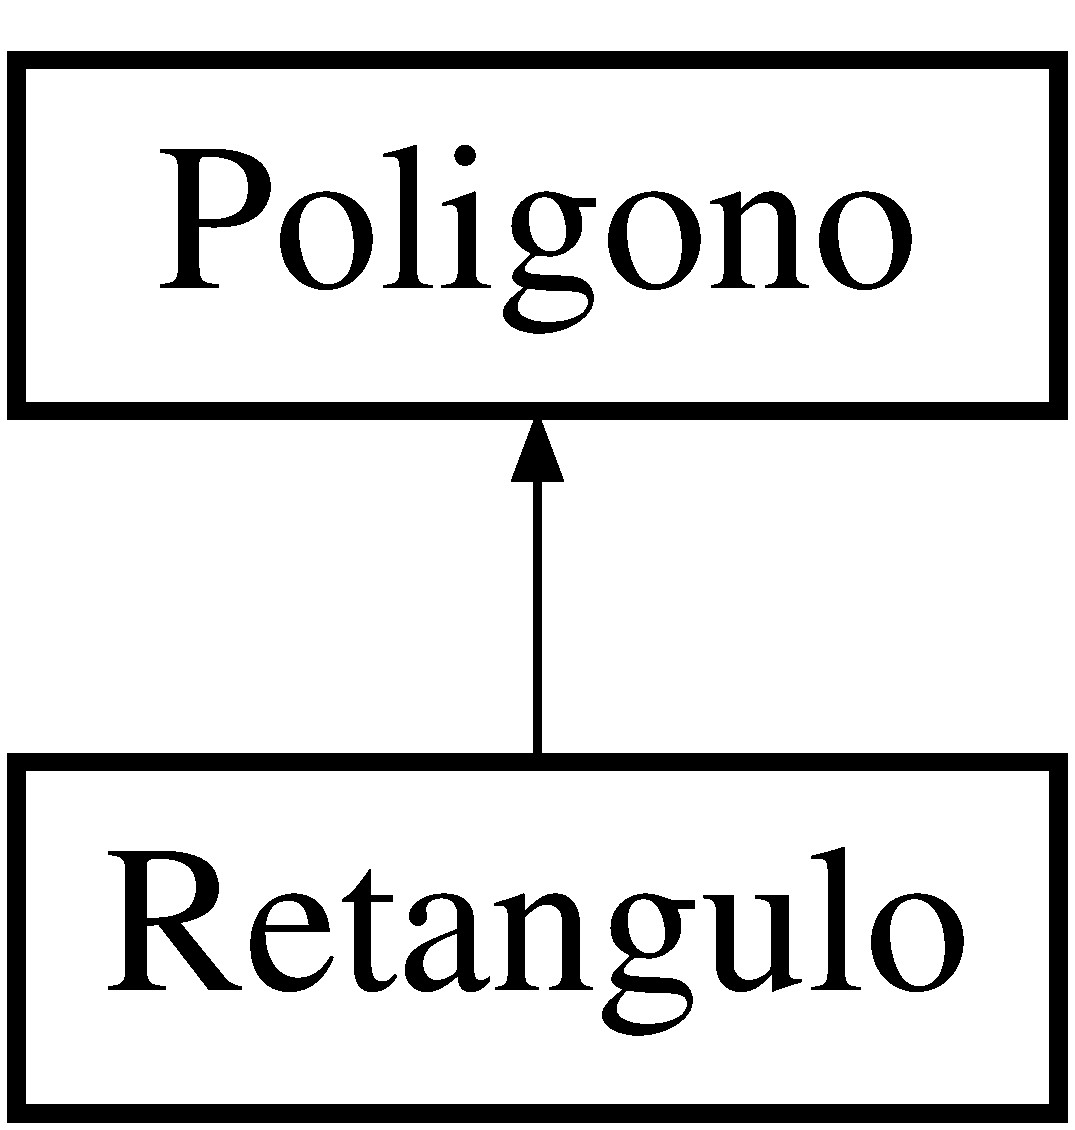
\includegraphics[height=2.000000cm]{class_poligono}
\end{center}
\end{figure}
\subsection*{Membros Públicos}
\begin{DoxyCompactItemize}
\item 
\textbf{ Poligono} ()
\begin{DoxyCompactList}\small\item\em \doxyref{Poligono\+::\+Poligono}{p.}{class_poligono_a9311a9a1496878c09c8508b3636e2870} -\/ Construtor da classe. \end{DoxyCompactList}\item 
void \textbf{ set\+Vertice} (float x, float y)
\begin{DoxyCompactList}\small\item\em \doxyref{Poligono\+::set\+Vertice}{p.}{class_poligono_a1d1ca86b608c4427bd39d3753230cc9b} -\/ Seta cada vertice(ponto) \end{DoxyCompactList}\item 
void \textbf{ quantidade} (void)
\begin{DoxyCompactList}\small\item\em \doxyref{Poligono\+::quantidade}{p.}{class_poligono_a3f4aa8038324ead841e04ffbbf6d8594} -\/ Retorna a quantidade de vertices ja inseridos. \end{DoxyCompactList}\item 
void \textbf{ imprimir\+Poli} (void)
\begin{DoxyCompactList}\small\item\em \doxyref{Poligono\+::imprimir\+Poli}{p.}{class_poligono_a0ee1c2c501af5df6fc844c7772696bc9} -\/ Imprime a estrutura do poligono usando para isso o metodo imprime() ja criado na classe \doxyref{Point}{p.}{class_point}. \end{DoxyCompactList}\item 
void \textbf{ area\+\_\+poligono} (void)
\begin{DoxyCompactList}\small\item\em \doxyref{Poligono\+::area\+\_\+poligono}{p.}{class_poligono_aee462c2f38ab2e1ca98f7ecee291ead8} -\/ Calculo da area do poligono usando para isso a tecnica shoelace. \end{DoxyCompactList}\item 
void \textbf{ translada\+Poli} (float \+\_\+a, float \+\_\+b)
\begin{DoxyCompactList}\small\item\em \doxyref{Poligono\+::translada\+Poli}{p.}{class_poligono_af79181410a3961117638e993321a67c2} -\/ Translada toda a estrutura do poligono usando para isso o metodo translada(\+\_\+a,\+\_\+b) ja implimentado na classe \doxyref{Point}{p.}{class_point}. \end{DoxyCompactList}\item 
void \textbf{ rotacionar} (float theta, float x, float y)
\begin{DoxyCompactList}\small\item\em \doxyref{Poligono\+::rotacionar}{p.}{class_poligono_a62edbbcf29d2b540999a1cd3cb4b1601} -\/ Rotaciona toda a estrutua do poligono. \end{DoxyCompactList}\end{DoxyCompactItemize}
\subsection*{Atributos Públicos}
\begin{DoxyCompactItemize}
\item 
\textbf{ Point} \textbf{ vertices} [100]
\item 
int \textbf{ n\+\_\+vertices} =0
\end{DoxyCompactItemize}


\subsection{Construtores e Destrutores}
\mbox{\label{class_poligono_a9311a9a1496878c09c8508b3636e2870}} 
\index{Poligono@{Poligono}!Poligono@{Poligono}}
\index{Poligono@{Poligono}!Poligono@{Poligono}}
\subsubsection{Poligono()}
{\footnotesize\ttfamily Poligono\+::\+Poligono (\begin{DoxyParamCaption}{ }\end{DoxyParamCaption})}



\doxyref{Poligono\+::\+Poligono}{p.}{class_poligono_a9311a9a1496878c09c8508b3636e2870} -\/ Construtor da classe. 



\subsection{Funções membros}
\mbox{\label{class_poligono_aee462c2f38ab2e1ca98f7ecee291ead8}} 
\index{Poligono@{Poligono}!area\+\_\+poligono@{area\+\_\+poligono}}
\index{area\+\_\+poligono@{area\+\_\+poligono}!Poligono@{Poligono}}
\subsubsection{area\+\_\+poligono()}
{\footnotesize\ttfamily void Poligono\+::area\+\_\+poligono (\begin{DoxyParamCaption}\item[{void}]{ }\end{DoxyParamCaption})}



\doxyref{Poligono\+::area\+\_\+poligono}{p.}{class_poligono_aee462c2f38ab2e1ca98f7ecee291ead8} -\/ Calculo da area do poligono usando para isso a tecnica shoelace. 

\mbox{\label{class_poligono_a0ee1c2c501af5df6fc844c7772696bc9}} 
\index{Poligono@{Poligono}!imprimir\+Poli@{imprimir\+Poli}}
\index{imprimir\+Poli@{imprimir\+Poli}!Poligono@{Poligono}}
\subsubsection{imprimir\+Poli()}
{\footnotesize\ttfamily void Poligono\+::imprimir\+Poli (\begin{DoxyParamCaption}\item[{void}]{ }\end{DoxyParamCaption})}



\doxyref{Poligono\+::imprimir\+Poli}{p.}{class_poligono_a0ee1c2c501af5df6fc844c7772696bc9} -\/ Imprime a estrutura do poligono usando para isso o metodo imprime() ja criado na classe \doxyref{Point}{p.}{class_point}. 

\mbox{\label{class_poligono_a3f4aa8038324ead841e04ffbbf6d8594}} 
\index{Poligono@{Poligono}!quantidade@{quantidade}}
\index{quantidade@{quantidade}!Poligono@{Poligono}}
\subsubsection{quantidade()}
{\footnotesize\ttfamily void Poligono\+::quantidade (\begin{DoxyParamCaption}\item[{void}]{ }\end{DoxyParamCaption})}



\doxyref{Poligono\+::quantidade}{p.}{class_poligono_a3f4aa8038324ead841e04ffbbf6d8594} -\/ Retorna a quantidade de vertices ja inseridos. 

\mbox{\label{class_poligono_a62edbbcf29d2b540999a1cd3cb4b1601}} 
\index{Poligono@{Poligono}!rotacionar@{rotacionar}}
\index{rotacionar@{rotacionar}!Poligono@{Poligono}}
\subsubsection{rotacionar()}
{\footnotesize\ttfamily void Poligono\+::rotacionar (\begin{DoxyParamCaption}\item[{float}]{theta,  }\item[{float}]{x,  }\item[{float}]{y }\end{DoxyParamCaption})}



\doxyref{Poligono\+::rotacionar}{p.}{class_poligono_a62edbbcf29d2b540999a1cd3cb4b1601} -\/ Rotaciona toda a estrutua do poligono. 


\begin{DoxyParams}{Parâmetros}
{\em theta} & -\/ Angulo para a rotação \\
\hline
{\em x} & -\/ Coordenda x do ponto central de rotação \\
\hline
{\em y} & -\/ Coordenda y do ponto central de rotação \\
\hline
\end{DoxyParams}
\mbox{\label{class_poligono_a1d1ca86b608c4427bd39d3753230cc9b}} 
\index{Poligono@{Poligono}!set\+Vertice@{set\+Vertice}}
\index{set\+Vertice@{set\+Vertice}!Poligono@{Poligono}}
\subsubsection{set\+Vertice()}
{\footnotesize\ttfamily void Poligono\+::set\+Vertice (\begin{DoxyParamCaption}\item[{float}]{x,  }\item[{float}]{y }\end{DoxyParamCaption})}



\doxyref{Poligono\+::set\+Vertice}{p.}{class_poligono_a1d1ca86b608c4427bd39d3753230cc9b} -\/ Seta cada vertice(ponto) 


\begin{DoxyParams}{Parâmetros}
{\em x} & -\/ Valor da coordenada x fornecida pelo usuario \\
\hline
{\em y} & -\/ Valor da coordenada y fornecida pelo usuario \\
\hline
\end{DoxyParams}
\mbox{\label{class_poligono_af79181410a3961117638e993321a67c2}} 
\index{Poligono@{Poligono}!translada\+Poli@{translada\+Poli}}
\index{translada\+Poli@{translada\+Poli}!Poligono@{Poligono}}
\subsubsection{translada\+Poli()}
{\footnotesize\ttfamily void Poligono\+::translada\+Poli (\begin{DoxyParamCaption}\item[{float}]{\+\_\+a,  }\item[{float}]{\+\_\+b }\end{DoxyParamCaption})}



\doxyref{Poligono\+::translada\+Poli}{p.}{class_poligono_af79181410a3961117638e993321a67c2} -\/ Translada toda a estrutura do poligono usando para isso o metodo translada(\+\_\+a,\+\_\+b) ja implimentado na classe \doxyref{Point}{p.}{class_point}. 


\begin{DoxyParams}{Parâmetros}
{\em \+\_\+a} & -\/ Unidade de translação da coordenada x \\
\hline
{\em \+\_\+b} & -\/ Unidade de translação da coordenada y \\
\hline
\end{DoxyParams}


\subsection{Atributos}
\mbox{\label{class_poligono_a284269050a0ce8fbe95e2c69b36c5709}} 
\index{Poligono@{Poligono}!n\+\_\+vertices@{n\+\_\+vertices}}
\index{n\+\_\+vertices@{n\+\_\+vertices}!Poligono@{Poligono}}
\subsubsection{n\+\_\+vertices}
{\footnotesize\ttfamily int Poligono\+::n\+\_\+vertices =0}

\mbox{\label{class_poligono_a18179d267bdf366f6bb00a4e1b16f1d7}} 
\index{Poligono@{Poligono}!vertices@{vertices}}
\index{vertices@{vertices}!Poligono@{Poligono}}
\subsubsection{vertices}
{\footnotesize\ttfamily \textbf{ Point} Poligono\+::vertices[100]}



A documentação para essa classe foi gerada a partir dos seguintes arquivos\+:\begin{DoxyCompactItemize}
\item 
\textbf{ poligono.\+h}\item 
\textbf{ poligono.\+cpp}\end{DoxyCompactItemize}

\section{Retangulo Class Reference}
\label{class_retangulo}\index{Retangulo@{Retangulo}}


{\ttfamily \#include $<$retangulo.\+h$>$}

Inheritance diagram for Retangulo\+:\begin{figure}[H]
\begin{center}
\leavevmode
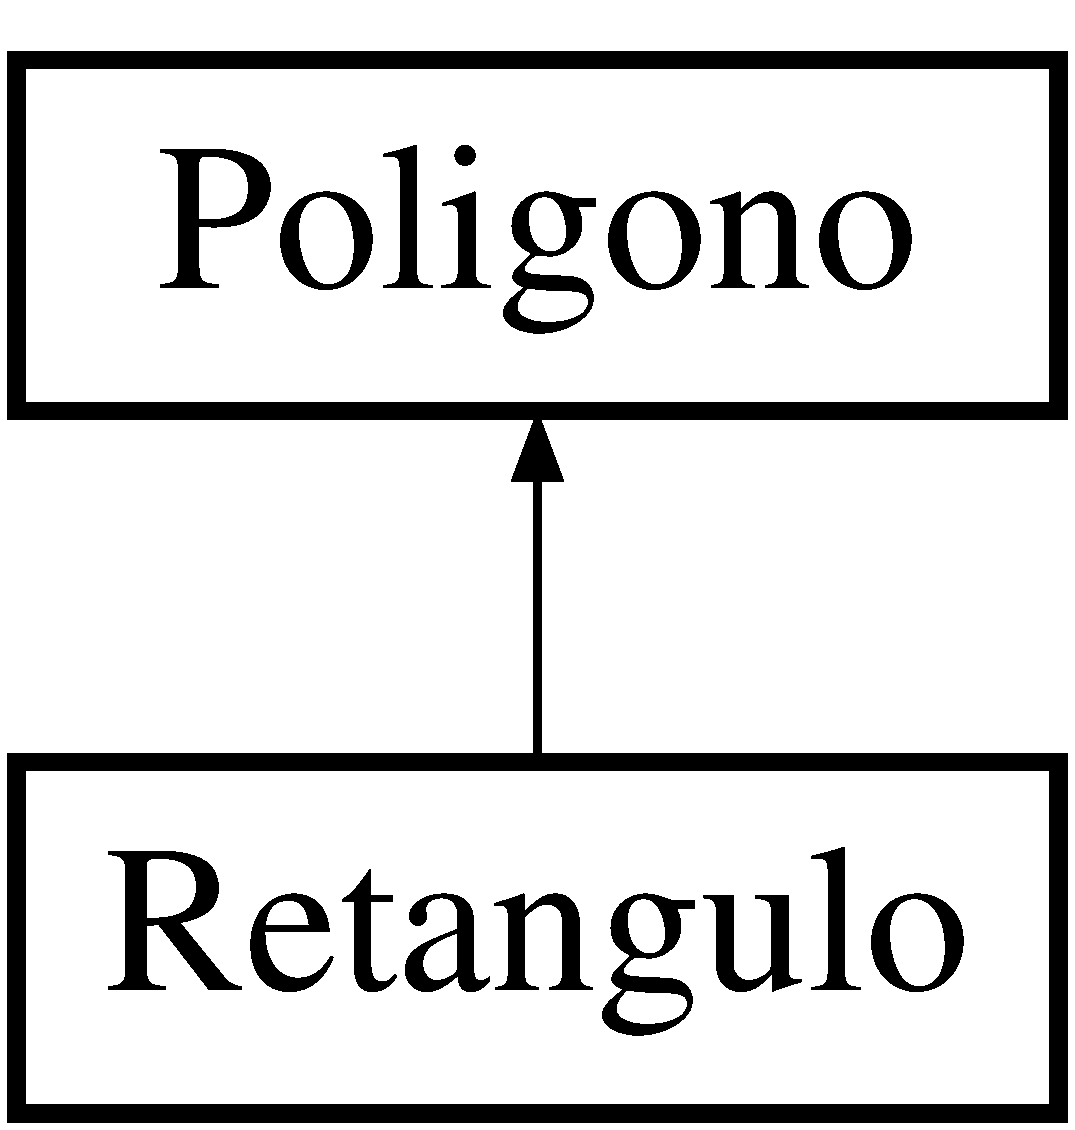
\includegraphics[height=2.000000cm]{class_retangulo}
\end{center}
\end{figure}
\subsection*{Public Member Functions}
\begin{DoxyCompactItemize}
\item 
\textbf{ Retangulo} (int x, int y, int larg, int alt, int aux)
\begin{DoxyCompactList}\small\item\em \doxyref{Retangulo\+::\+Retangulo}{p.}{class_retangulo_a5533c28fd6bf3dba362565351c2883dc} -\/ Construtor da classe retangulo. \end{DoxyCompactList}\item 
virtual void \textbf{ draw} (\textbf{ Screen} \&t)
\begin{DoxyCompactList}\small\item\em \doxyref{Retangulo\+::draw}{p.}{class_retangulo_ac088dd6d3f4f3d3f80363a868c2e74f1} -\/ Desenha o retangulo de acordo com o algoritmo implementado. \end{DoxyCompactList}\end{DoxyCompactItemize}


\subsection{Constructor \& Destructor Documentation}
\mbox{\label{class_retangulo_a5533c28fd6bf3dba362565351c2883dc}} 
\index{Retangulo@{Retangulo}!Retangulo@{Retangulo}}
\index{Retangulo@{Retangulo}!Retangulo@{Retangulo}}
\subsubsection{Retangulo()}
{\footnotesize\ttfamily Retangulo\+::\+Retangulo (\begin{DoxyParamCaption}\item[{int}]{\+\_\+x,  }\item[{int}]{\+\_\+y,  }\item[{int}]{\+\_\+larg,  }\item[{int}]{\+\_\+alt,  }\item[{int}]{\+\_\+aux }\end{DoxyParamCaption})}



\doxyref{Retangulo\+::\+Retangulo}{p.}{class_retangulo_a5533c28fd6bf3dba362565351c2883dc} -\/ Construtor da classe retangulo. 


\begin{DoxyParams}{Parameters}
{\em \+\_\+x} & -\/ Coordenada x onde o retangulo sera iniciado \\
\hline
{\em \+\_\+y} & -\/ Coordenada y onde o retangulo sera iniciado \\
\hline
{\em \+\_\+larg} & -\/ Largura do retangulo \\
\hline
{\em \+\_\+alt} & -\/ Altura do retangulo \\
\hline
{\em \+\_\+aux} & -\/ Variavel responsavel por verificar se o retangulo sera preenchido ou não \\
\hline
\end{DoxyParams}


\subsection{Member Function Documentation}
\mbox{\label{class_retangulo_ac088dd6d3f4f3d3f80363a868c2e74f1}} 
\index{Retangulo@{Retangulo}!draw@{draw}}
\index{draw@{draw}!Retangulo@{Retangulo}}
\subsubsection{draw()}
{\footnotesize\ttfamily void Retangulo\+::draw (\begin{DoxyParamCaption}\item[{\textbf{ Screen} \&}]{t }\end{DoxyParamCaption})\hspace{0.3cm}{\ttfamily [virtual]}}



\doxyref{Retangulo\+::draw}{p.}{class_retangulo_ac088dd6d3f4f3d3f80363a868c2e74f1} -\/ Desenha o retangulo de acordo com o algoritmo implementado. 


\begin{DoxyParams}{Parameters}
{\em t} & -\/ Desenha o retangulo na tela(matriz) \\
\hline
\end{DoxyParams}


Implements \textbf{ Figura\+Geometrica} \doxyref{}{p.}{class_figura_geometrica_a8ee8dedc060b6059a805ea091aef2c41}.



The documentation for this class was generated from the following files\+:\begin{DoxyCompactItemize}
\item 
\textbf{ retangulo.\+h}\item 
\textbf{ retangulo.\+cpp}\end{DoxyCompactItemize}

\chapter{Arquivos}
\section{main.\+cpp File Reference}
\label{main_8cpp}\index{main.\+cpp@{main.\+cpp}}
{\ttfamily \#include \char`\"{}mainwindow.\+h\char`\"{}}\newline
{\ttfamily \#include $<$Q\+Application$>$}\newline
\subsection*{Functions}
\begin{DoxyCompactItemize}
\item 
int \textbf{ main} (int argc, char $\ast$argv[$\,$])
\end{DoxyCompactItemize}


\subsection{Function Documentation}
\mbox{\label{main_8cpp_a0ddf1224851353fc92bfbff6f499fa97}} 
\index{main.\+cpp@{main.\+cpp}!main@{main}}
\index{main@{main}!main.\+cpp@{main.\+cpp}}
\subsubsection{main()}
{\footnotesize\ttfamily int main (\begin{DoxyParamCaption}\item[{int}]{argc,  }\item[{char $\ast$}]{argv[$\,$] }\end{DoxyParamCaption})}


\section{Referência do Arquivo point.\+cpp}
\label{point_8cpp}\index{point.\+cpp@{point.\+cpp}}
{\ttfamily \#include \char`\"{}point.\+h\char`\"{}}\newline
{\ttfamily \#include $<$cmath$>$}\newline
{\ttfamily \#include $<$iostream$>$}\newline

\section{Referência do Arquivo point.\+h}
\label{point_8h}\index{point.\+h@{point.\+h}}
\subsection*{Componentes}
\begin{DoxyCompactItemize}
\item 
class \textbf{ Point}
\end{DoxyCompactItemize}

\section{Referência do Arquivo poligono.\+cpp}
\label{poligono_8cpp}\index{poligono.\+cpp@{poligono.\+cpp}}
{\ttfamily \#include \char`\"{}poligono.\+h\char`\"{}}\newline
{\ttfamily \#include \char`\"{}point.\+h\char`\"{}}\newline
{\ttfamily \#include $<$cmath$>$}\newline
{\ttfamily \#include $<$iostream$>$}\newline

\section{Referência do Arquivo poligono.\+h}
\label{poligono_8h}\index{poligono.\+h@{poligono.\+h}}
{\ttfamily \#include \char`\"{}point.\+h\char`\"{}}\newline
\subsection*{Componentes}
\begin{DoxyCompactItemize}
\item 
class \textbf{ Poligono}
\end{DoxyCompactItemize}

\section{retangulo.\+cpp File Reference}
\label{retangulo_8cpp}\index{retangulo.\+cpp@{retangulo.\+cpp}}
{\ttfamily \#include \char`\"{}retangulo.\+h\char`\"{}}\newline
{\ttfamily \#include \char`\"{}reta.\+h\char`\"{}}\newline

\section{retangulo.\+h File Reference}
\label{retangulo_8h}\index{retangulo.\+h@{retangulo.\+h}}
{\ttfamily \#include $<$figurageometrica.\+h$>$}\newline
\subsection*{Classes}
\begin{DoxyCompactItemize}
\item 
class \textbf{ Retangulo}
\end{DoxyCompactItemize}

%--- End generated contents ---

% Index
\backmatter
\newpage
\phantomsection
\clearemptydoublepage
\addcontentsline{toc}{chapter}{Sumário}
\printindex

\end{document}
